\documentclass[a4paper, 10pt]{article}
\usepackage[utf8]{inputenc}
\usepackage{geometry}
\usepackage{polski}
\usepackage{graphicx}
\usepackage{float}
\usepackage{etoolbox,refcount}
\usepackage{multicol}
\usepackage{fancyhdr}
\usepackage{amsfonts}
\usepackage{listings}
\usepackage{amsmath}
\usepackage{svg}
\usepackage{pdfpages}

\newgeometry{left=2.5cm, right=2.5cm, bottom=2.5cm, top=2.5cm}
\title{Optymalizacja parametryczna}
\author{Adrian Jałoszewski}
\date{16 maja 2017}
\begin{document}
    \maketitle
	\section{Cel ćwiczenia}
		Celem ćwiczenia jest dokonanie optymalizacji nastaw regulatora PID w celu minimalizacji uchybu regulacji w układzie ujemnego sprzężenia zwrotnego stosując różne wskaźniki jakości.
	\section{Przebieg ćwiczenia}
		Ćwiczenie polegało na dobraniu regulatora PID minimalizującego pewien współczynnik jakości dla regulacji w sprzężeniu zwrotnym obiektu o transmitancji: 
		$$
			G(s) = \frac{1}{(Ts + 1)^n}
		$$
		Gdzie $n$ to miesiąc urodzin, a $T$ to odwrotność dnia urodzin. W moim przypadku ten szczęśliwy dzień przypadł na jedenastego sierpnia.
		\begin{figure}[H]
			\centering
			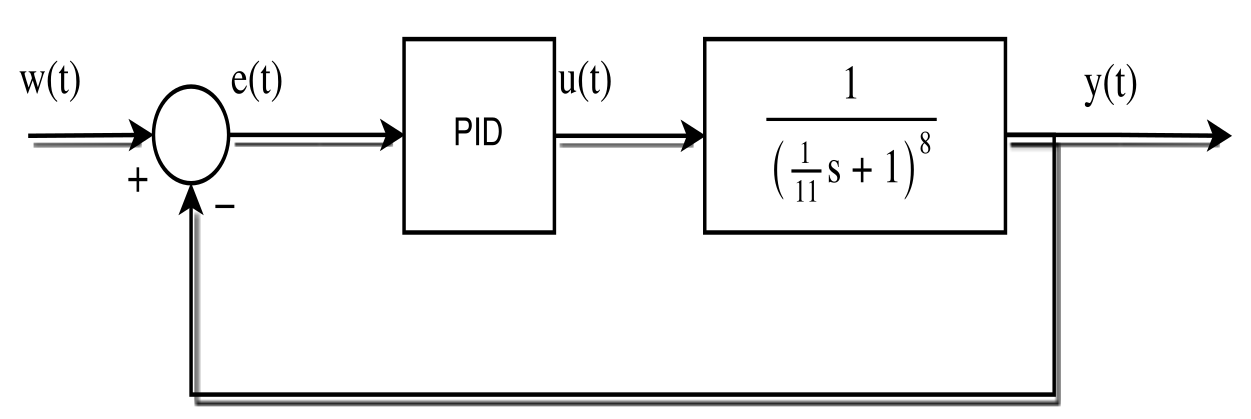
\includegraphics[width =0.8\columnwidth]{schemat.png}
			\caption{Układ regulacji}
		\end{figure} \noindent
		Badany był uchyb regulacji w przypadku podania na wejście układu skoku jednostkowego.
		\subsection{Całka z uchybu}
			Dosyć naiwnym wskaźnikiem jakości regulacji jest minimalizacja:
			$$
				J = \int_0^\infty
				e(t) \mathrm{d}t
			$$
			Problem leży w tym, że całka ta dla tego układu ma minimum dla nastaw dla których układ jest niestabilny. Nastawy regulacji są wtedy dobierane tak, żeby wskaźnik był ujemny, co skutkuje tym, że co raz więcej co raz głębszych dołków zmniejsza wartość całki.
		\subsection{Całka z modułu z uchybu}
			Wadą tego wskaźnika jest to, że jest nieróżniczkowalny. Traktuje również podobnie uchyby duże i małe, co sprawia, że na wykresach wizualnie zdaje się dawać najlepszy wynik - jest to minimalizacja powierzchni między krzywą, a osią odciętych.
			$$
				J = \int_0^\infty
				|e(t)| \mathrm{d}t
			$$
			\begin{figure}[H]
				\centering
				\def \svgwidth{0.65\columnwidth}
				\input{abs.pdf_tex}
				\caption{Wartość uchybu}
			\end{figure}\noindent
		\subsection{Całka z kwadratu z uchybu}
			Wskaźnik ten eksponuje bardziej uchyby duże niż małe. Wynika to z tego, że gdy $a > b > 0$, to
			$\frac{a}{b} < \left(\frac{a}{b}\right)^2$. Dlatego też sprowadza uchyb z początku szybciej do zera, skutkując następnie większymi przeregulowaniami.
			$$
				J = \int_0^\infty
				e^2(t) \mathrm{d}t
			$$
			\begin{figure}[H]
				\centering
				\def \svgwidth{0.65\columnwidth}
				\input{square.pdf_tex}
				\caption{Wartość uchybu}
			\end{figure}\noindent
		\subsection{Całka z kwadratu uchybu z czasem jako waga}
			Wskaźnik ten eksponuje bardziej uchyby późniejsze niż wcześniejsze -- uchyb jest mniejszy później.
			$$
				J = \int_0^\infty
				te^2(t) \mathrm{d}t
			$$
			\begin{figure}[H]
				\centering
				\def \svgwidth{0.65\columnwidth}
				\input{linear.pdf_tex}
				\caption{Wartość uchybu}
			\end{figure}\noindent
		\subsection{Całka z sumy kwadratu uchybu i kwadratu jego pierwszej pochodnej}
			Wskaźnik ten minimalizuje również szybkość zmiany uchybu, jednak aby zmusić uchyb do zmierzania do zera jest dodany czynnik pomniejszający uchyb.
			$$
				J = \int_0^\infty
				e^2(t) + \dot{e}^2(t)\mathrm{d}t
			$$
			\begin{figure}[H]
				\centering
				\def \svgwidth{0.65\columnwidth}
				\input{rate_change.pdf_tex}
				\caption{Wartość uchybu}
			\end{figure}\noindent
		\subsection{Porównanie wskaźników}
			\begin{figure}[H]
				\centering
				\def \svgwidth{\columnwidth}
				\input{cumulative.pdf_tex}
				\caption{Porównanie wskaźników}
			\end{figure}f\noindent
			\begin{itemize}
				\item[] Całka z uchybu -- brak na wykresie, ponieważ nie generowała wyników dla których układ byłby stabilny
				\item[] Całka z kwadratu uchybu -- minimalizuje czas dojścia uchybu do zera
				\item[] Całka z modułu uchybu - najmniejsze pole powierzchni między osią odciętych, a uchybem
				\item[] Całka z kwadratu uchybu z czasem jako waga -- z czasem jest bliżej zera niż w pozostałych przypadkach
				\item[] Całka z sumy kwadratu uchybu i kwadratu jego pierwszej pochodnej -- najwolniej opada
			\end{itemize}
	\section{Wnioski i obserwacje}
		Niektóre wskaźniki są gorsze od pozostałych, gdyż nie generują wyników, dla których układ byłby stabilny -- tak jak w tym przypadku całka z uchybu. Pozostałe rozważane przypadki natomiast mogą mieć zastosowanie w swoich dziedzinach i są używaniem odpowiedniego narzędzia do odpowiedniego zadania. Wskaźnik minimalizujący szybkość zmian nie będzie się nadawał do ramienia grającego w pingponga, a wskaźnik preferujący szybką zmianę dużego uchybu nie będzie się nadawał do przenoszenia fiolek nitrogliceryny. Przewaga wskaźnika stosującego czas jako wagę byłaby prawdopodobnie lepiej widoczna na obiekcie posiadającym pierwiastki zespolone nierzeczywiste (charakter oscylacyjny).
		\\ \\
		W niektórych przypadkach wymagana była zmiana solvera, gdyż np. domyślny solver pakietu scipy nie działał dla przypadku z modułem (był to solver oparty na jednym z algorytmów gradientowych, zastosowany został zamiast niego algorytm Powella).
\end{document}
